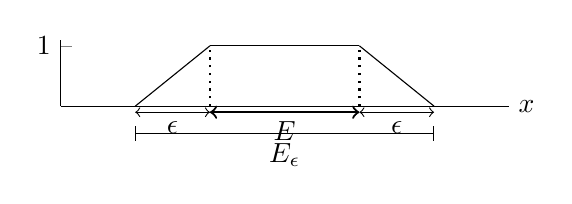
\begin{tikzpicture}
    \begin{axis}[
    axis lines*=left,
    clip = false,
    xmin = 0, xmax = 1, 
    ymin = 0, ymax = 1.1, 
    xtick = \empty, 
    ytick = {1},
    yticklabels={$1$}, 
    axis lines* = left,
    width=0.6\textwidth, height=0.2\textwidth]
    \addplot[domain=1/6:1/3] {6*(x-1/6)};
    \addplot[domain=1/3:2/3] {1};
    \addplot[domain=2/3:5/6] {6*(5/6-x)};
    \addplot[mark=none, black, thick, dotted] coordinates {(1/3,0) (1/3,1)};
    \addplot[mark=none, black, thick, dotted] coordinates {(2/3,0) (2/3,1)};
    \node [right] at (current axis.right of origin){$x$};
    \draw[<->, thick] (1/3, -0.1) to (2/3, -0.1);
    \draw[<->] (1/6, -0.1) to (1/3, -0.1);
    \draw[<->] (2/3, -0.1) to (5/6, -0.1);
    \draw[|-|] (1/6, -0.45) to (5/6, -0.45);
    \node [below] at (1/4, -0.1) {$\epsilon$};
    \node [below] at (3/4, -0.1) {$\epsilon$};
    \node [below] at (1/2, -0.1) {$E$};
    \node [below] at (1/2, -0.45) {$E_\epsilon$};
    \end{axis}
\end{tikzpicture}